% !TEX TS-program = xelatex
% !TEX encoding = UTF-8
% !Mode:: "TeX:UTF-8"

\documentclass[onecolumn,oneside]{SUSTechHomework}

\usepackage{float}

\author{胡玉斌}
\sid{11712121}
\title{Lab 6}
\coursecode{CS315}
\coursename{Computer Security}

\begin{document}
  \maketitle

  \section{Lab 6 Part 1}

    \subsection{Read the lab instructions above and finish all the tasks.}

    Done

    \subsection{Answer the questions in the Introduction section, and justify your answers. Simple yes or no answer will not get any credits.}

      \subsubsection{What security features does Zephyr have?}

        \begin{itemize}
          \item The security functionality in Zephyr hinges mainly on the inclusion of cryptographic algorithms, and on its monolithic system design.
          \item The security architecture is based on a monolithic design where the Zephyr kernel and all applications are compiled into a single static binary. System calls are implemented as function calls without requiring context switches. Static linking eliminates the potential for dynamically loading malicious code.
          \item Stack protection mechanisms are provided to protect against stack overruns.
        \end{itemize}

      \subsubsection{Do applications share the same address space with the OS kernel?}

        \begin{itemize}
          \item No
          \item It is very dangerous to share the the same address space with the OS kernel which means we can modify the value in that address space.
        \end{itemize}

      \subsubsection{Does Zephyr have defense mechanisms such as non-executable stack or Address Space Layout Randomization (ASLR)?}

        \begin{itemize}
          \item No
          \item Due to the exploration, we can see that the EIP register has the same value for the same payload and generate the special value for the EIP register.
          \item So Zephyr do not defense mechanisms.
        \end{itemize}

      \subsubsection{Do textbook attacks(e.g., buffer overflow or heap spray)work on Zephyr?}

        \begin{itemize}
          \item Yes
          \item Due to the exploration, we generate a payload to cause the buffer overflow. 
          \item As we expected, the application crashes due to an invalid return address.
          \item Furthermore, QEMU also crashes and you will see a pop-up window as the screenshot below.
        \end{itemize}

    \subsection{Change the EIP register to the value 0xdeadbeef, and show me the screenshot of the EIP value when the application crashes.}

      \begin{figure}[H]
        \centering
        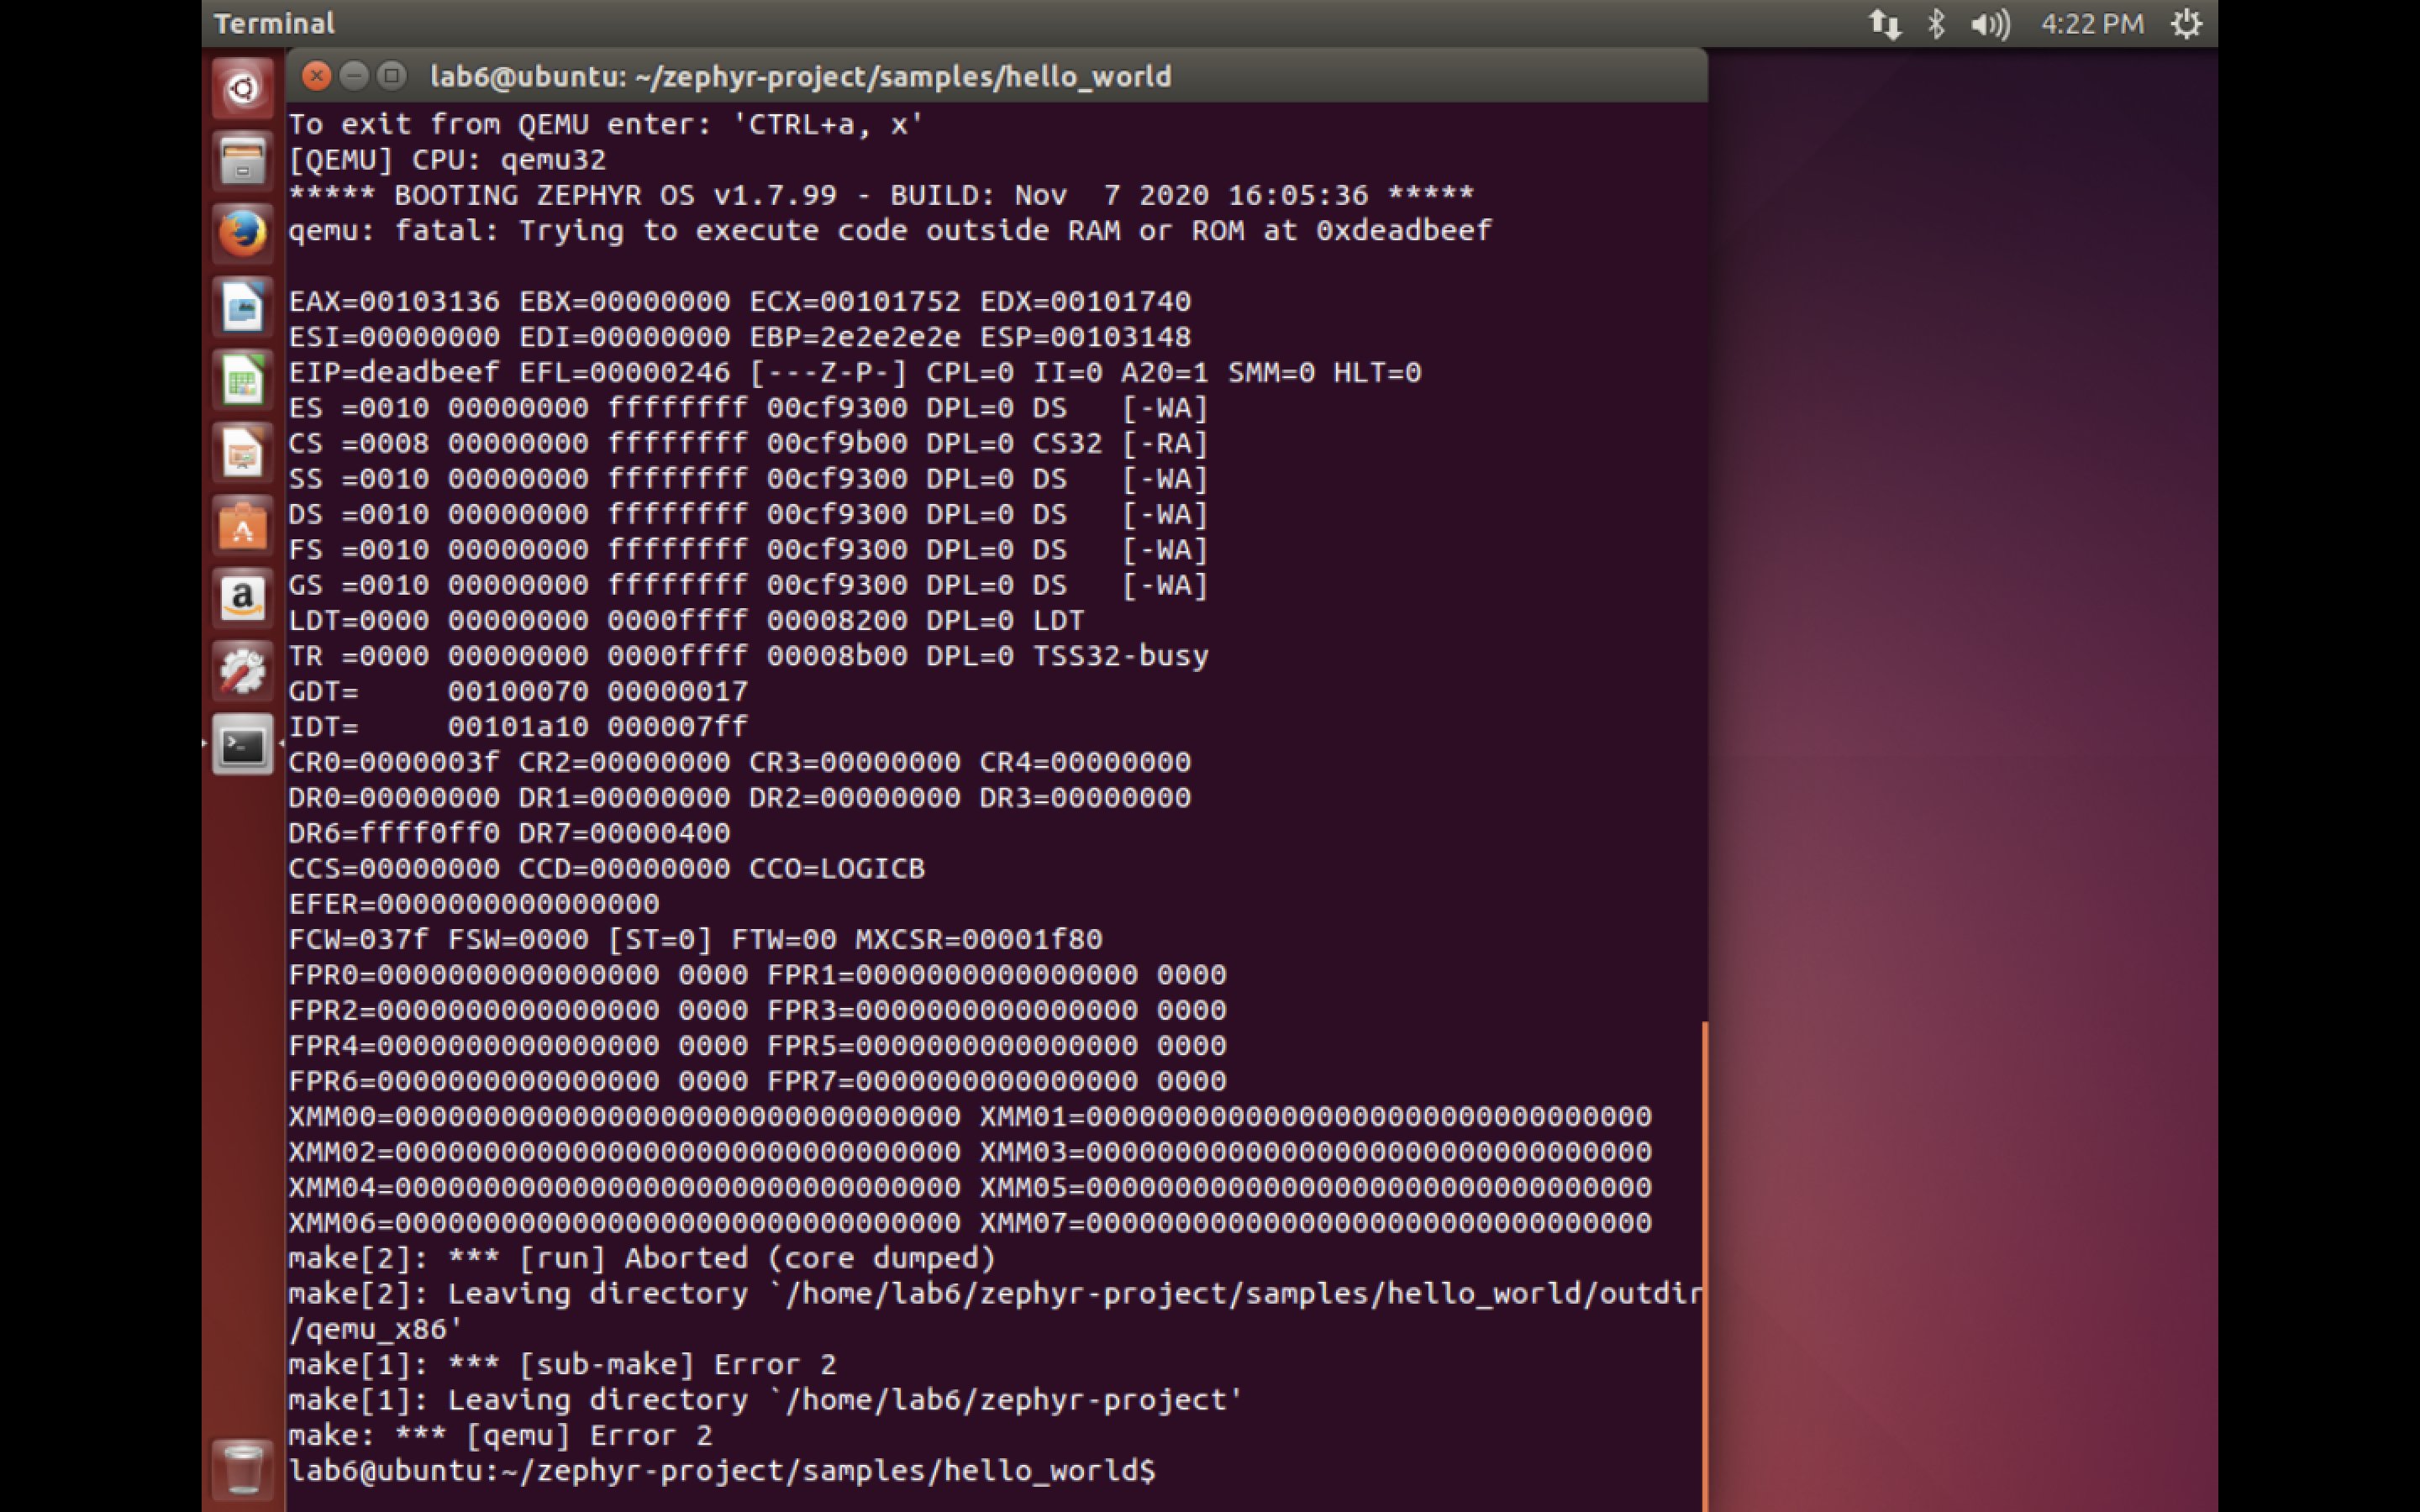
\includegraphics[width=0.95\textwidth]{img/pic1.png}
        \caption{EIP value}
      \end{figure}

      \begin{figure}[H]
        \centering
        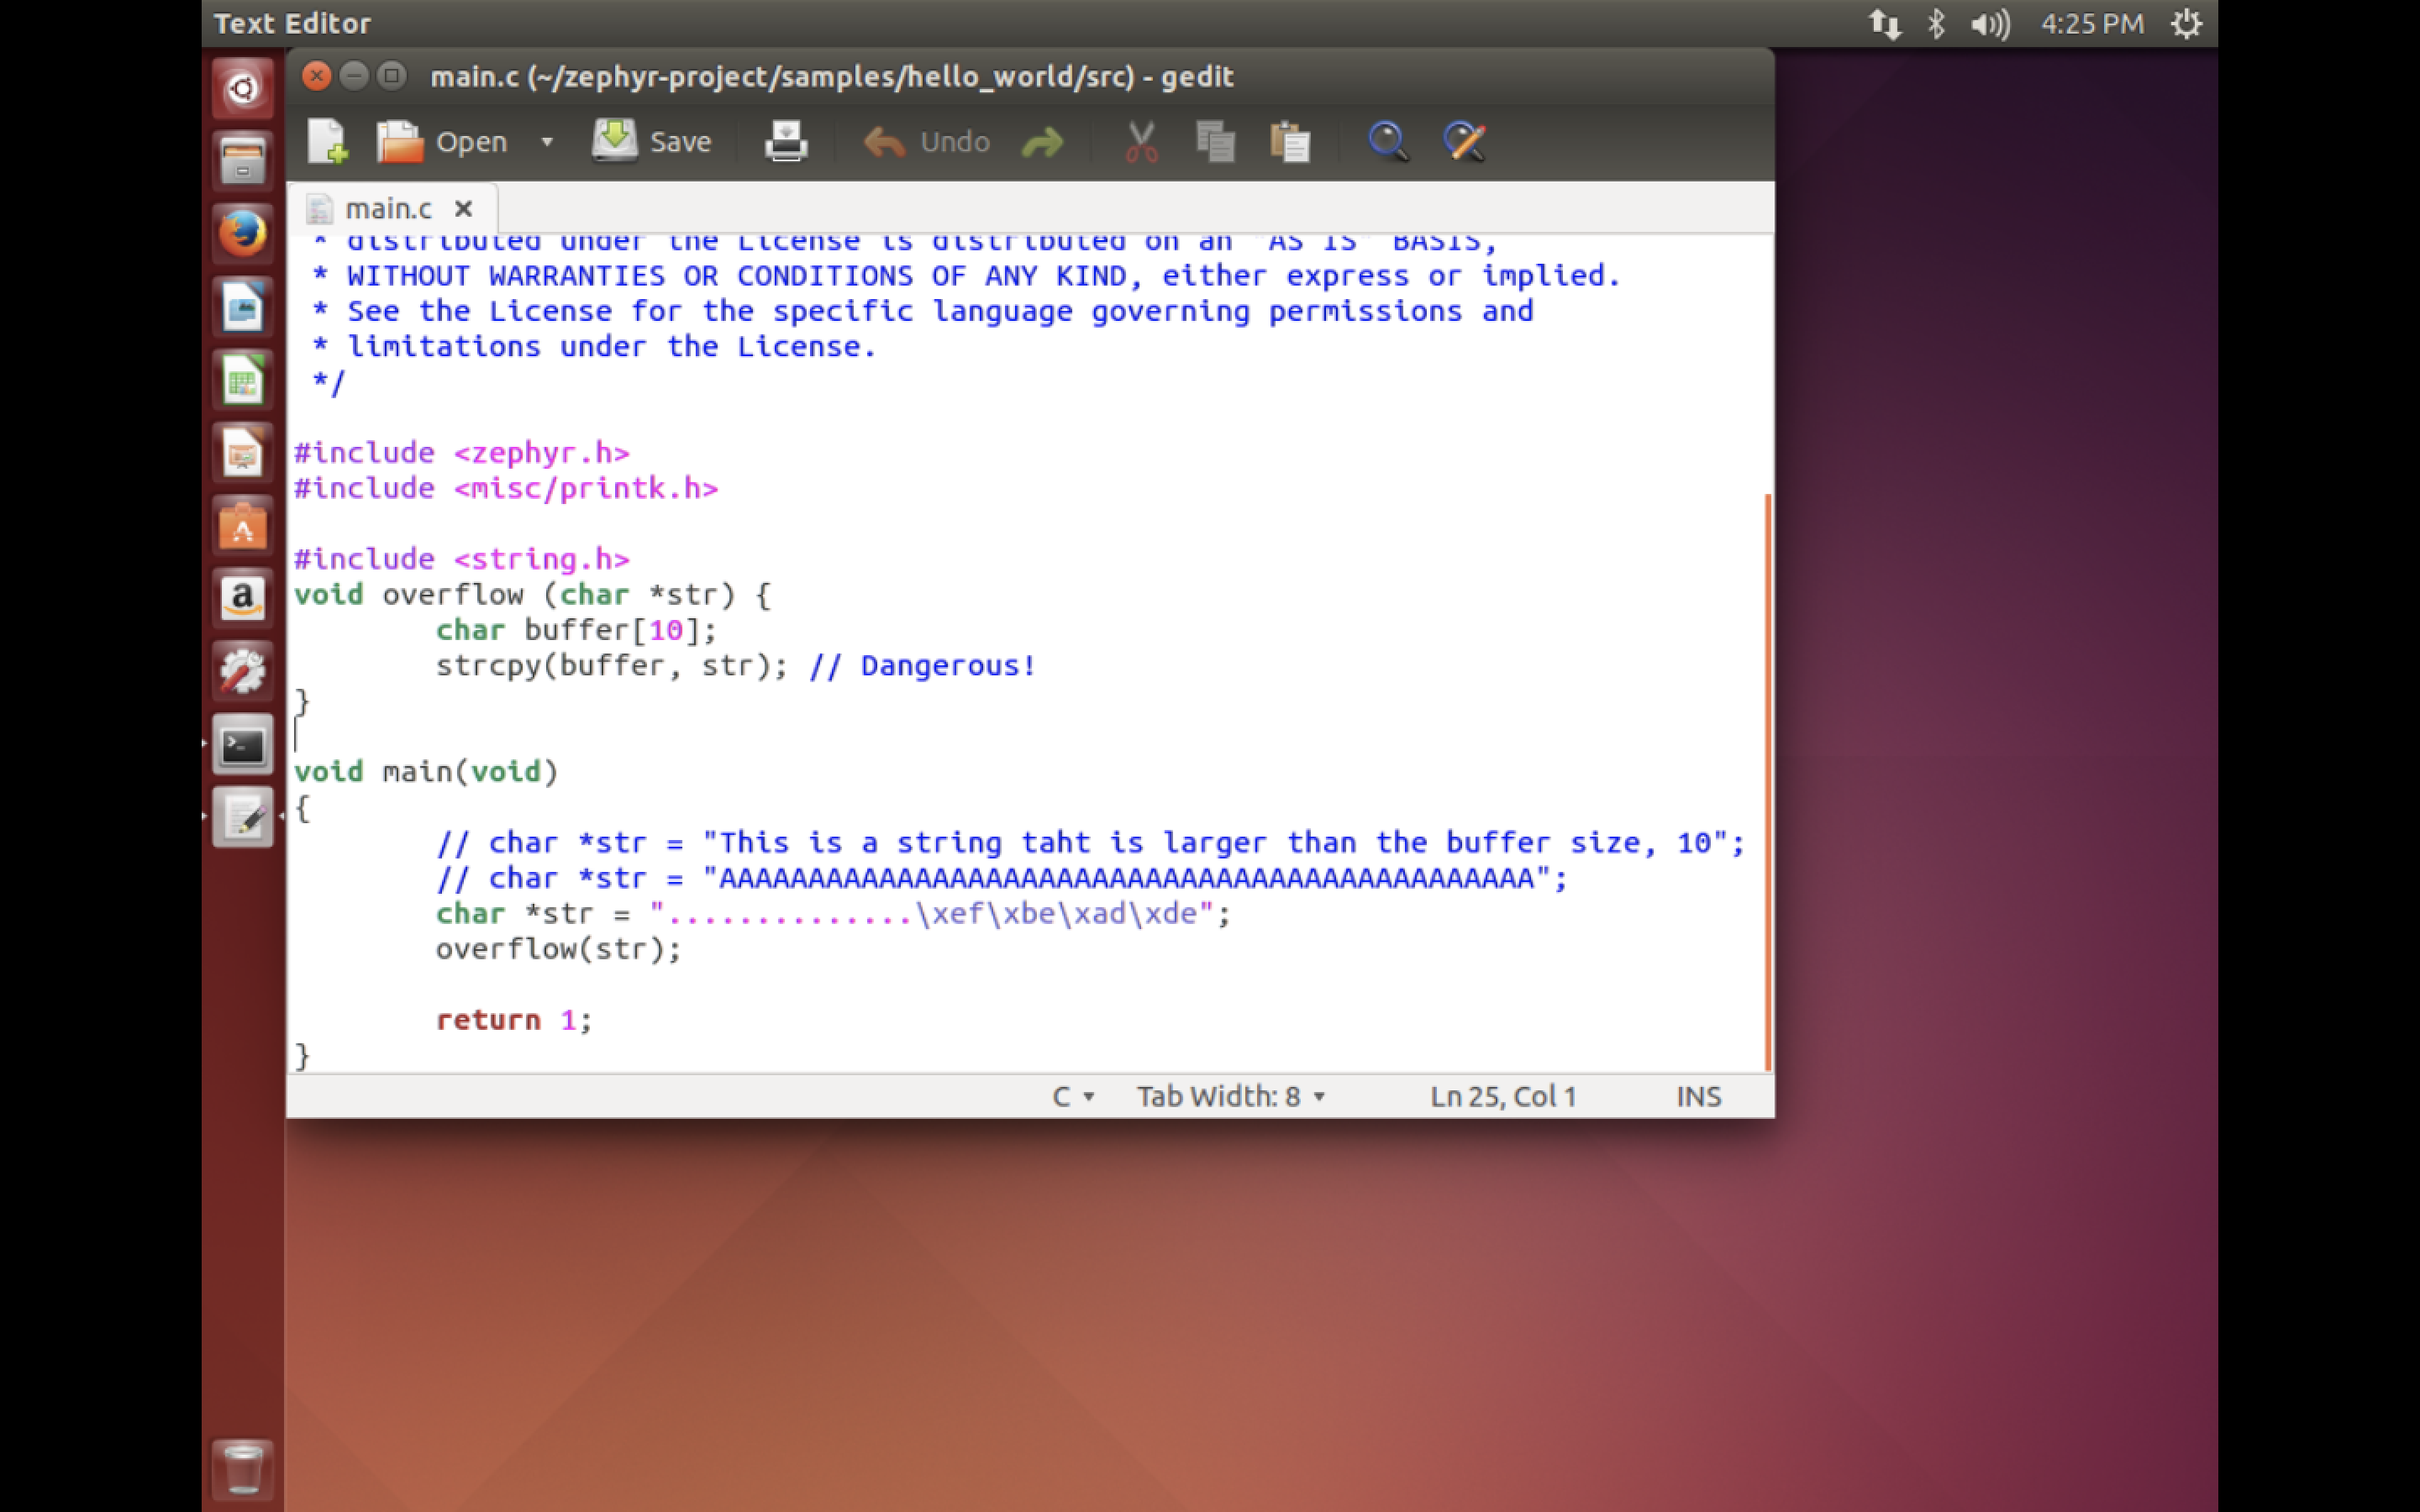
\includegraphics[width=0.95\textwidth]{img/pic2.png}
        \caption{obfuscate}
      \end{figure}

  \section{Lab 6 Part 2}

    \subsection{Read the lab instructions above and finish all the tasks.}

    Done

    \subsection{Answer the questions in the Introduction section,and justify your answers. Simple yes or no answer will not get any credits.}

      \subsubsection{What is the difference between Monitor Mode and Promiscuous Mode}

      \begin{itemize}
        \item Monitor mode: Sniffing the packets in the air without connecting (associating) with any access point.
        \item Promiscuous mode: Sniffing the packets after connecting to an access point. This is possible because the wireless-enabled devices send the data in the air but only "mark" them to be processed by the intended receiver. They cannot send the packets and make sure they only reach a specific device, unlike with switched LANs.
      \end{itemize}

      \subsubsection{What lessons we learned from this lab about setting the WiFi password?}

      \begin{itemize}
        \item We should use strong password.
        \item Avoid using weak password to be blasted by weak password tables.
      \end{itemize}

    \subsection{Change your router to a different pass phrase, and use the Wireshark and Aircrach-ng to crack the passphrase. Show screenshots of the result.}

    Use airport command to enable monitor mode, and monitor on channel 6.

    The password of the router is \textbf{SUSTech-Eveneko}

      \begin{figure}[H]
        \centering
        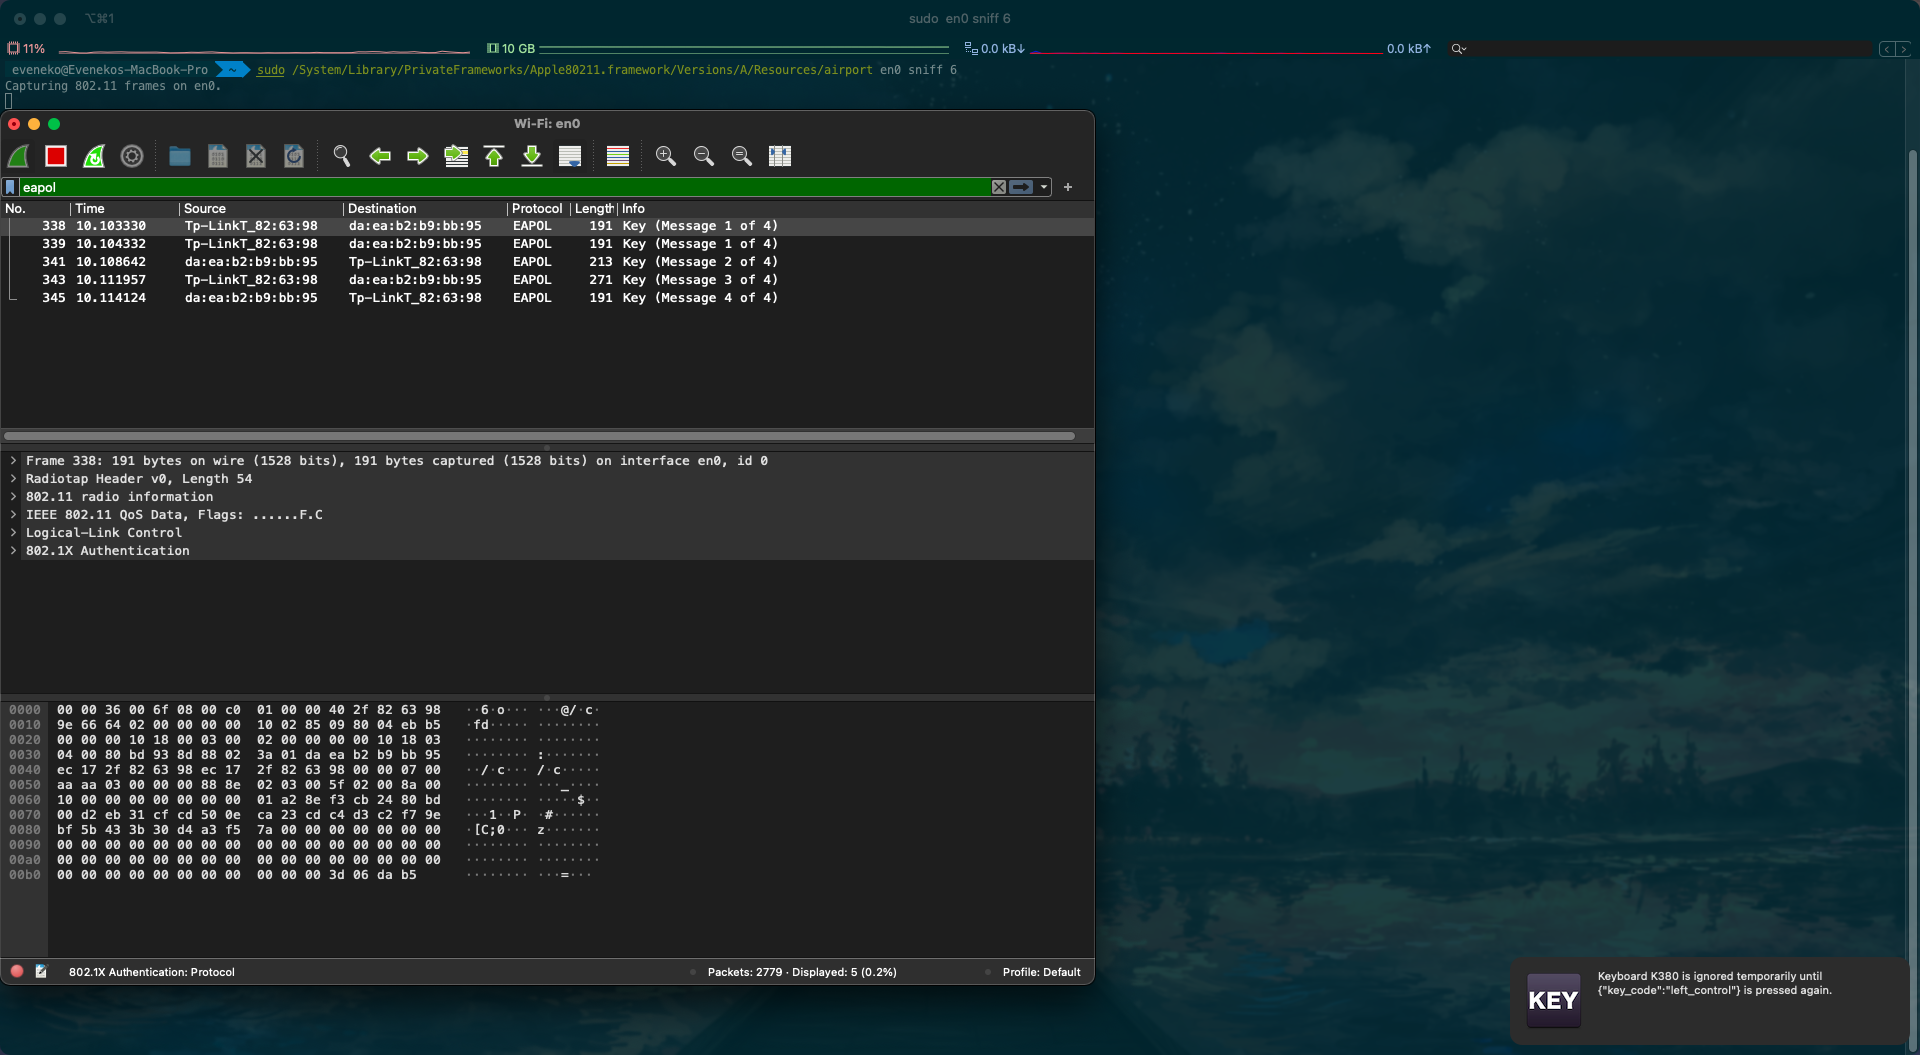
\includegraphics[width=0.95\textwidth]{img/pic3.png}
        \caption{Wireshark}
      \end{figure}

      \begin{figure}[H]
        \centering
        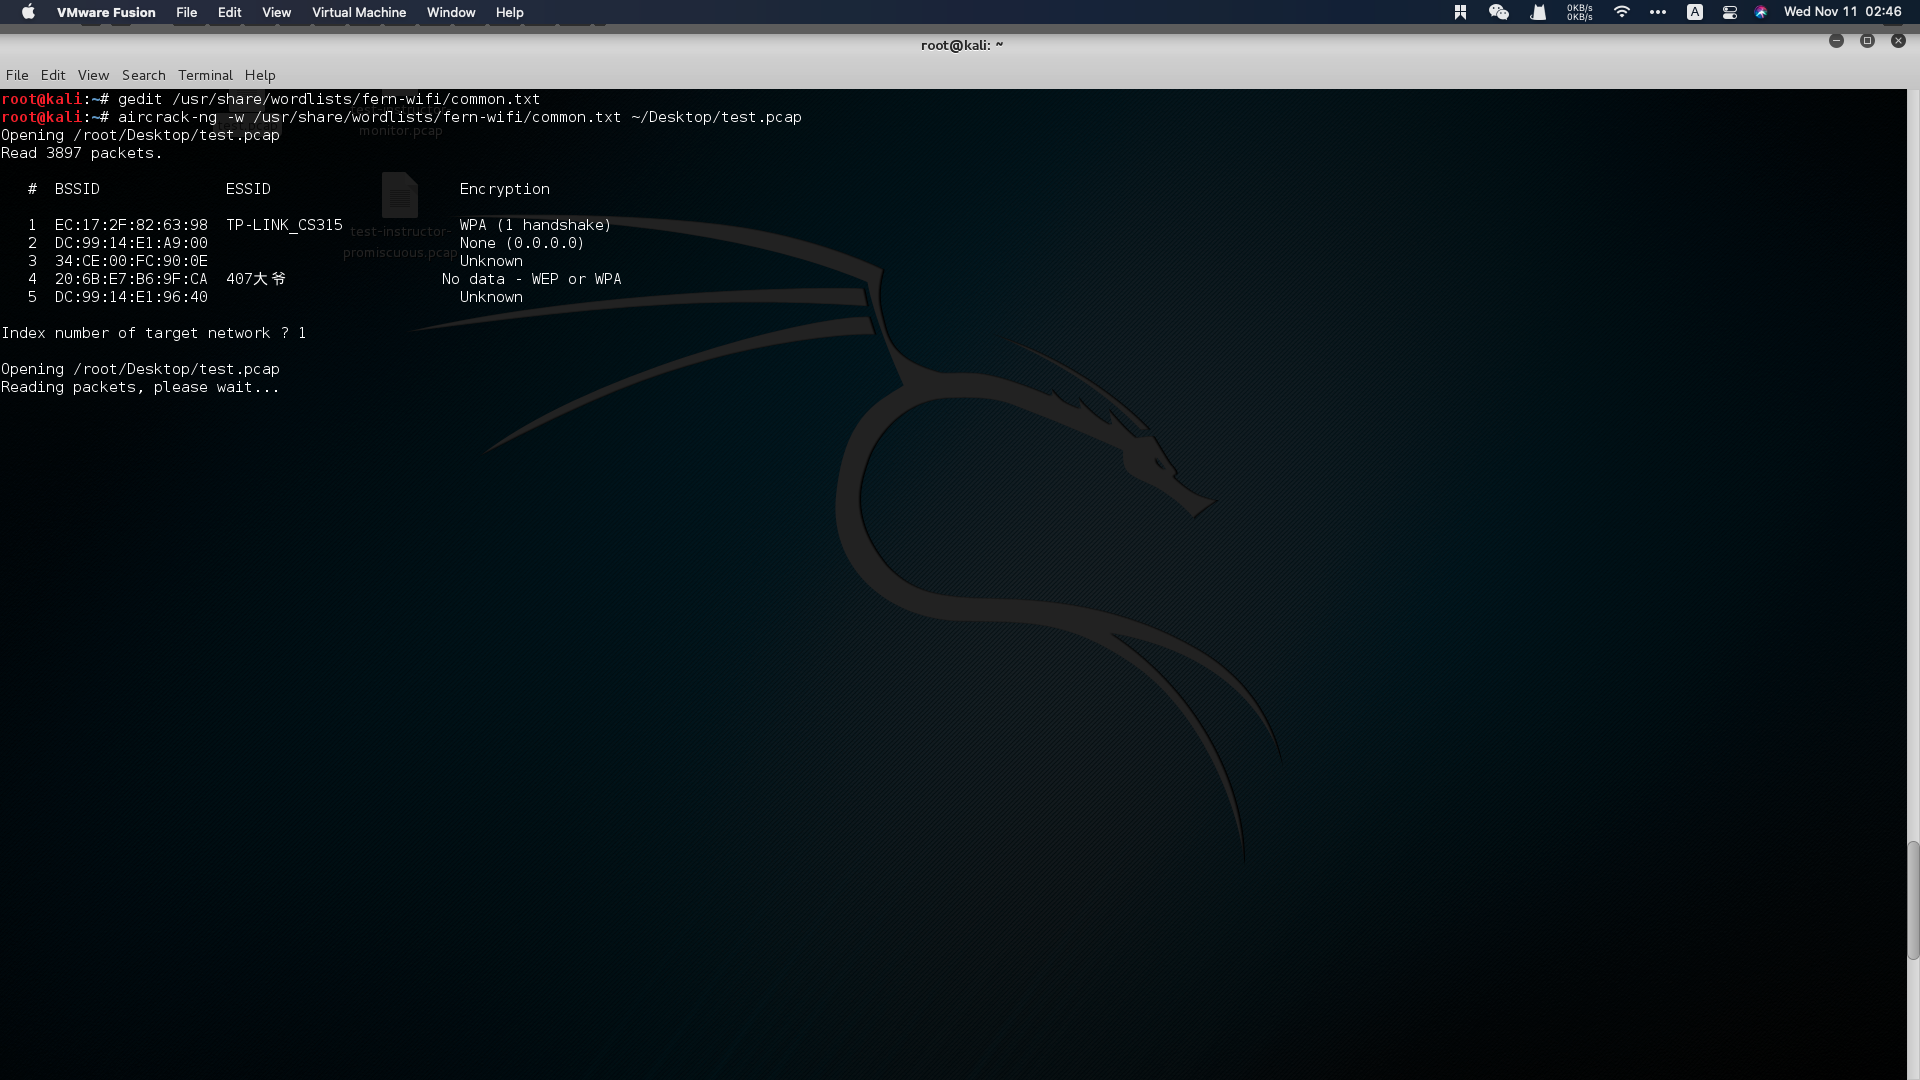
\includegraphics[width=0.95\textwidth]{img/pic4.png}
        \caption{password1}
      \end{figure}

      \begin{figure}[H]
        \centering
        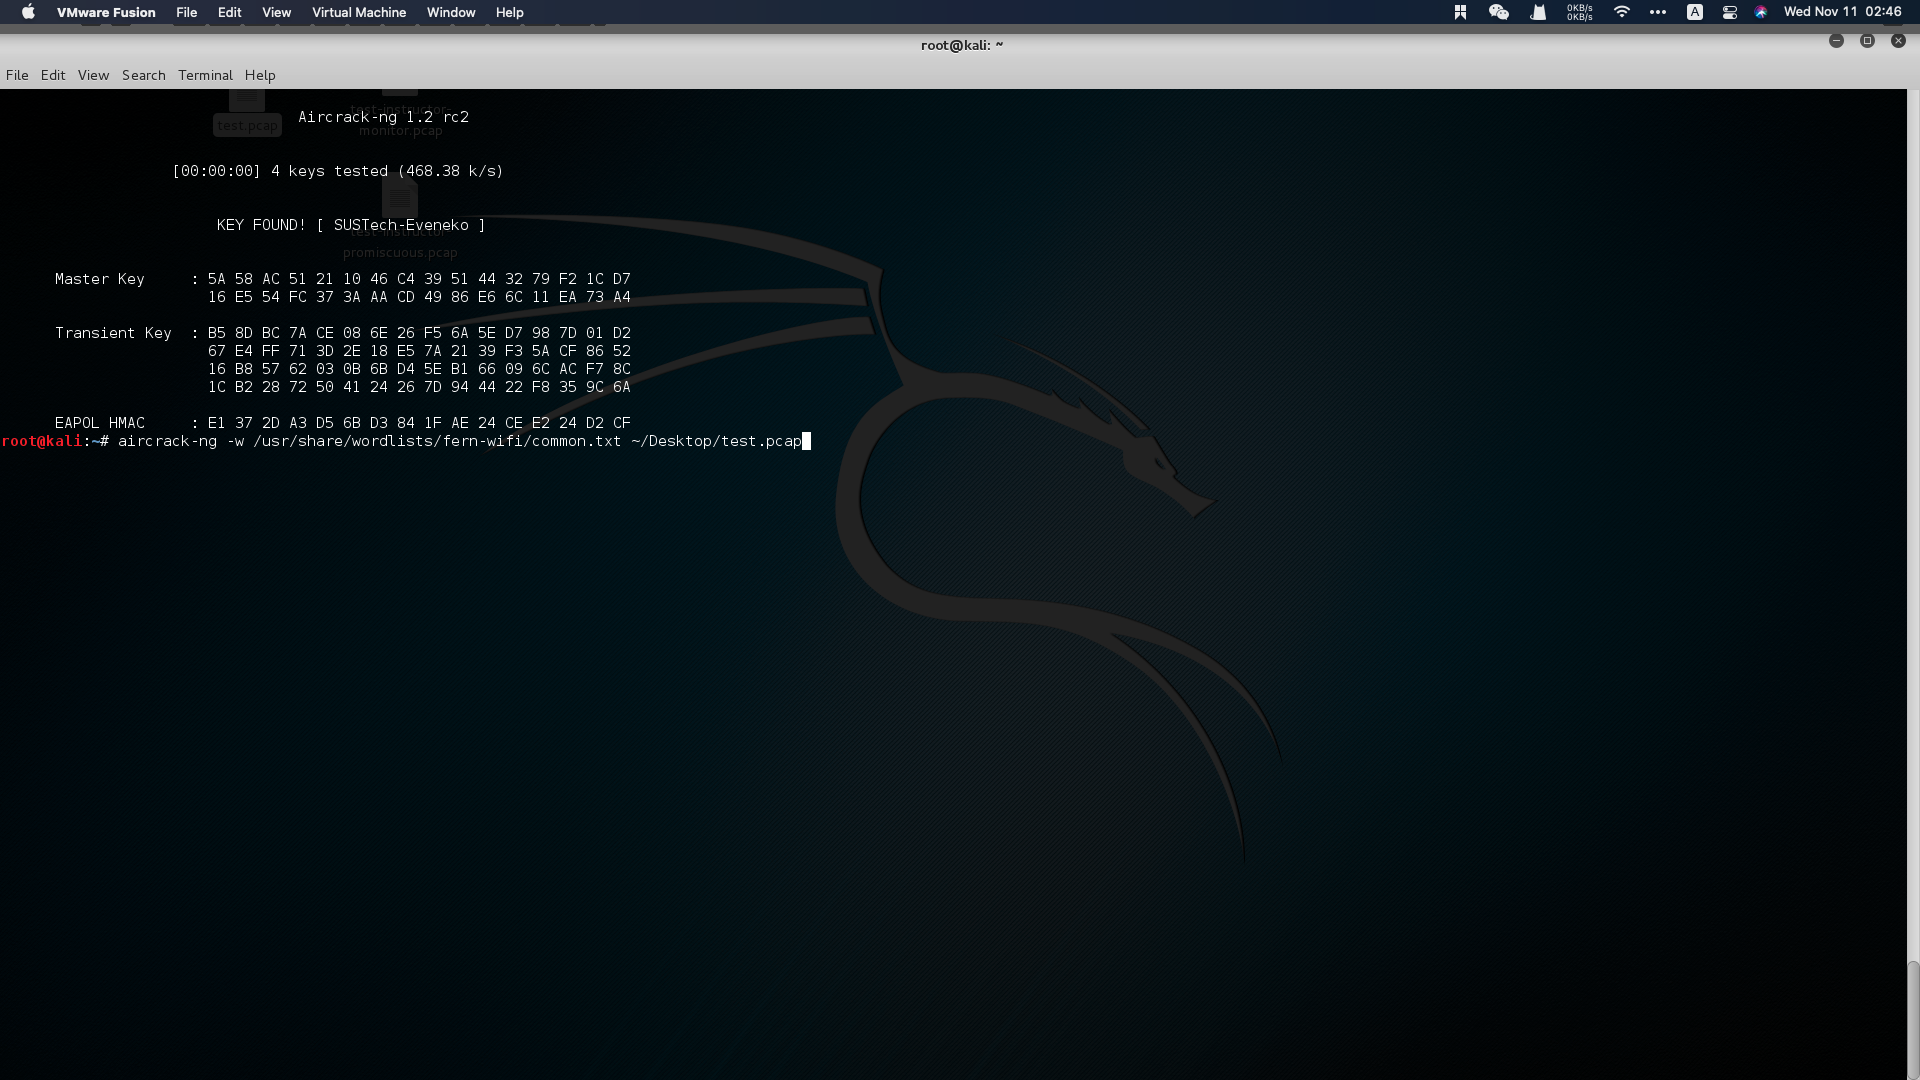
\includegraphics[width=0.95\textwidth]{img/pic5.png}
        \caption{password2}
      \end{figure}

\end{document}
